\documentclass[a4paper,14pt]{extarticle} 
\usepackage[a4paper,top=1.5cm, bottom=1.5cm, left=2cm, right=1cm]{geometry}
%\usepackage[T2A]{fontenc}
%\usepackage[english, russian]{babel}
\usepackage{graphicx}
\DeclareGraphicsExtensions{.pdf,.png,.jpg}

\usepackage{fontspec}
\setmainfont{Times New Roman}
\setsansfont{FreeSans}
\setmonofont{FreeMono}
\renewcommand{\baselinestretch}{1.5}
\usepackage{polyglossia}
\setdefaultlanguage{russian}
\setotherlanguages{english,russian}
\usepackage{setspace}
\usepackage[many]{tcolorbox}

\begin{document}
    \begin{center}
        \thispagestyle{empty}
        \begin{singlespace}
        МИНИСТЕРСТВО ЦИФРОВОГО РАЗВИТИЯ, СВЯЗИ И МАССОВЫХ КОММУНИКАЦИЙ РОССИЙСКОЙ ФЕДЕРАЦИИ

        ФЕДЕРАЛЬНОЕ ГОСУДАРСТВЕННОЕ БЮДЖЕТНОЕ ОБРАЗОВАТЕЛЬНОЕ

        УЧРЕЖДЕНИЕ ВЫСШЕГО ОБРАЗОВАНИЯ

        «САНКТ-ПЕТЕРБУРГСКИЙ ГОСУДАРСТВЕННЫЙ УНИВЕРСИТЕТ ТЕЛЕКОММУНИКАЦИЙ ИМ. ПРОФ. М.А. БОНЧ-БРУЕВИЧА»

        (СПбГУТ)
        \end{singlespace}
        \vspace{-1ex}
        \rule{\textwidth}{0.4pt}
        \vspace{-5ex}

        Факультет \underline{Инфокоммуникационных сетей и систем}

        Кафедра \underline{Защищенных систем связи}
        \vspace{10ex}

        \textbf{Лабораторная работа №13}\\
        Исследование криптосистем с открытым ключом


    \end{center}
    \vspace{4ex}
    \begin{flushright}
    \parbox{10 cm}{
    \begin{flushleft}
        Выполнил студент группы ИКТЗ-83:

        \underline{Громов А.А. } \hfill \rule[-0.85ex]{0.1\textwidth}{0.6pt}

        \footnotesize \textit{ (Ф.И.О., № группы) \hfill (подпись)} \normalsize

        Проверил:

        \underline{Яковлев В.А.} \hfill \rule[-0.85ex]{0.1\textwidth}{0.6pt}

        (\footnotesize \textit{уч. степень, уч. звание, Ф.И.О.) \hfill (подпись)} \normalsize

    \end{flushleft}
    }
    \end{flushright}
    \begin{center}
        \vfill
        Санкт-Петербург

        2021

    \end{center}
    \newpage

    \textbf{Цель лабораторной работы:} \par
    Приобретение навыков анализа алгоритмов криптосистем с открытыми ключами.

    \begin{center}
        \textbf{Текст 1}
    \end{center}

    \begin{center}
        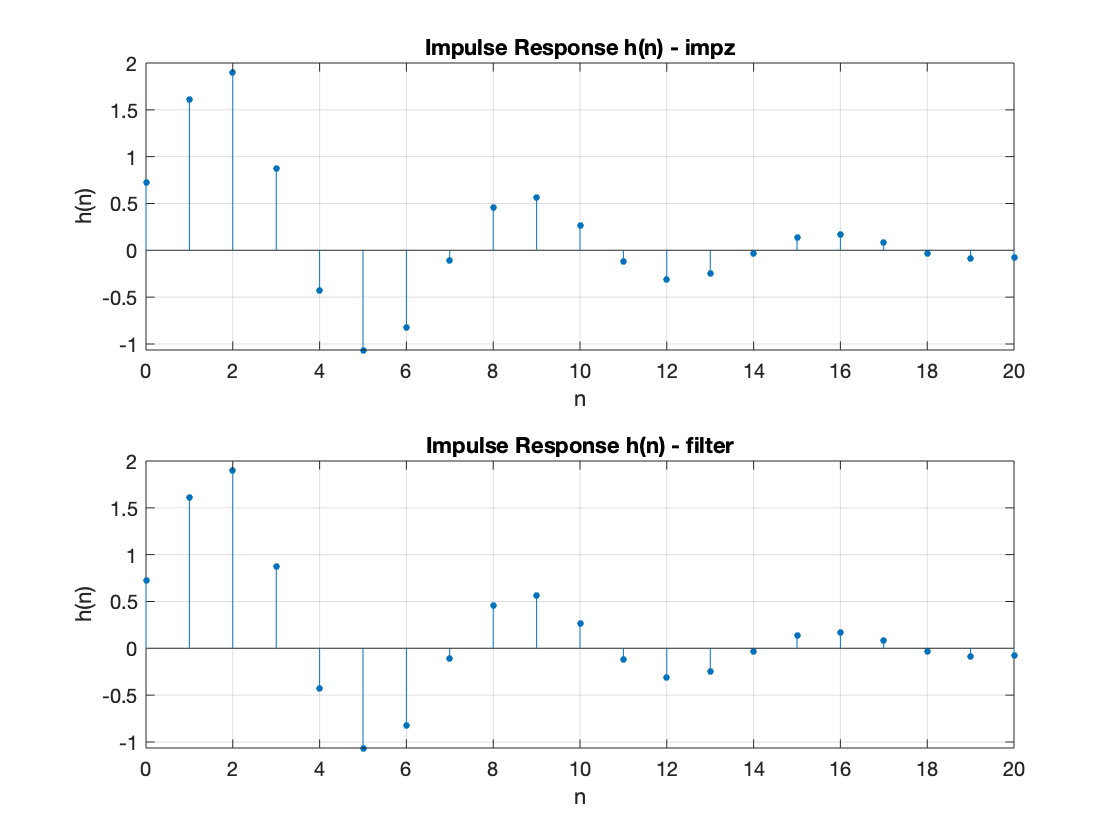
\includegraphics[scale=0.3]{pics/1.png}

        "Текст 1, зашифрованный"
    \end{center}
    \begin{center}
        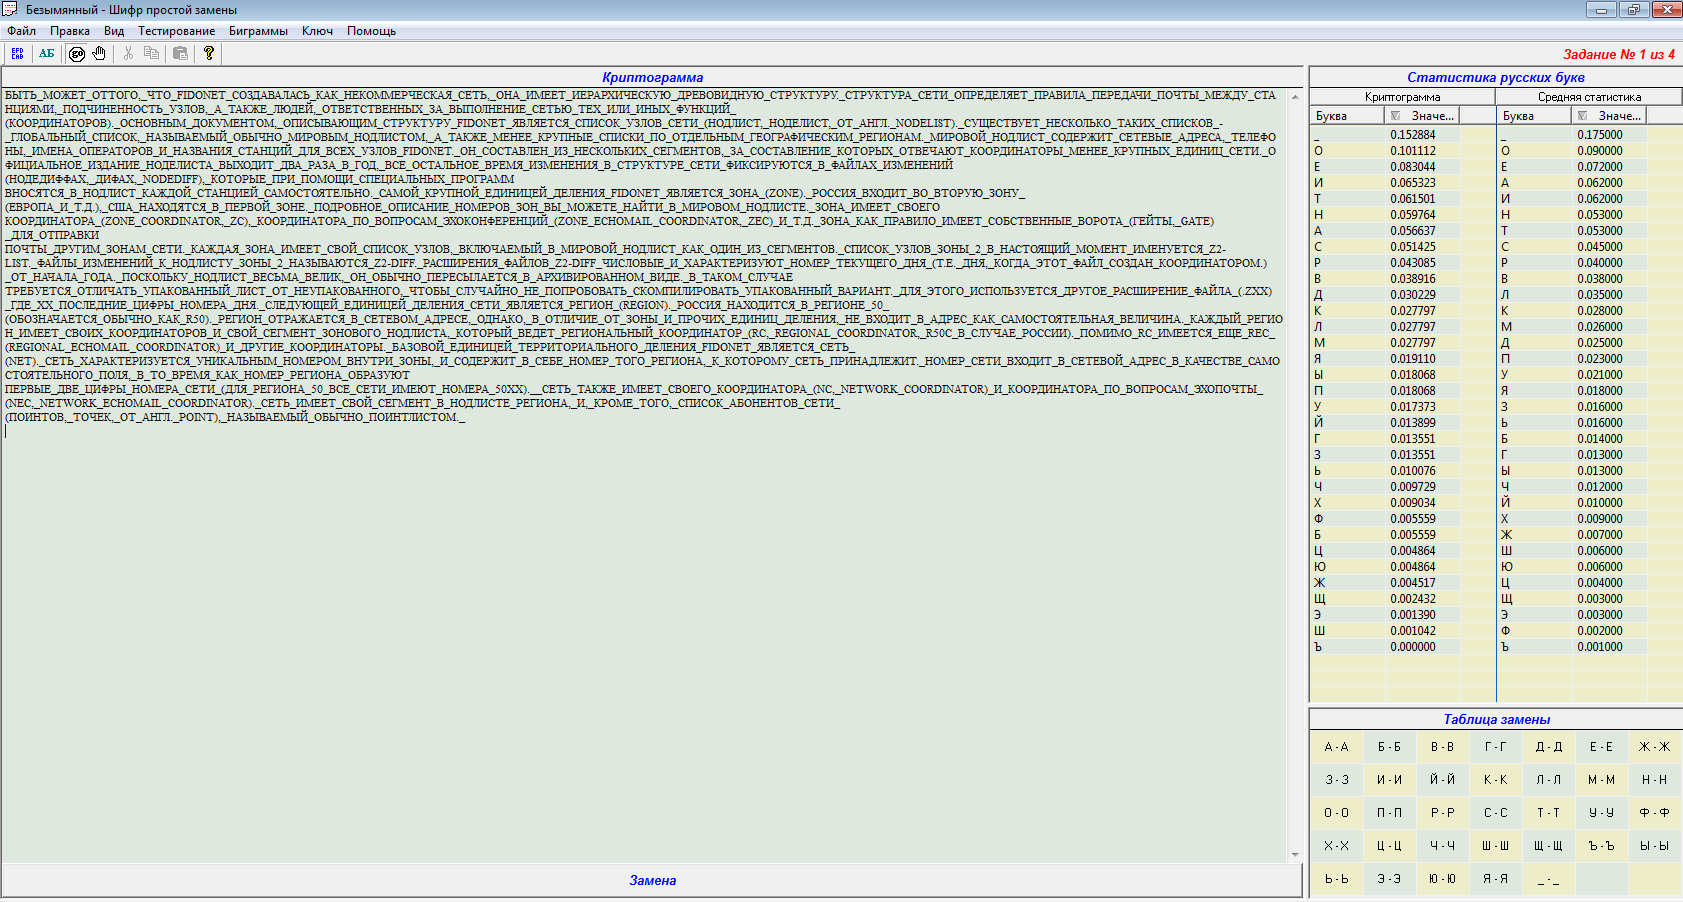
\includegraphics[scale=0.3]{pics/1_1.png}

        "Текст 1, расшифрованный"
    \end{center}
    \begin{center}
        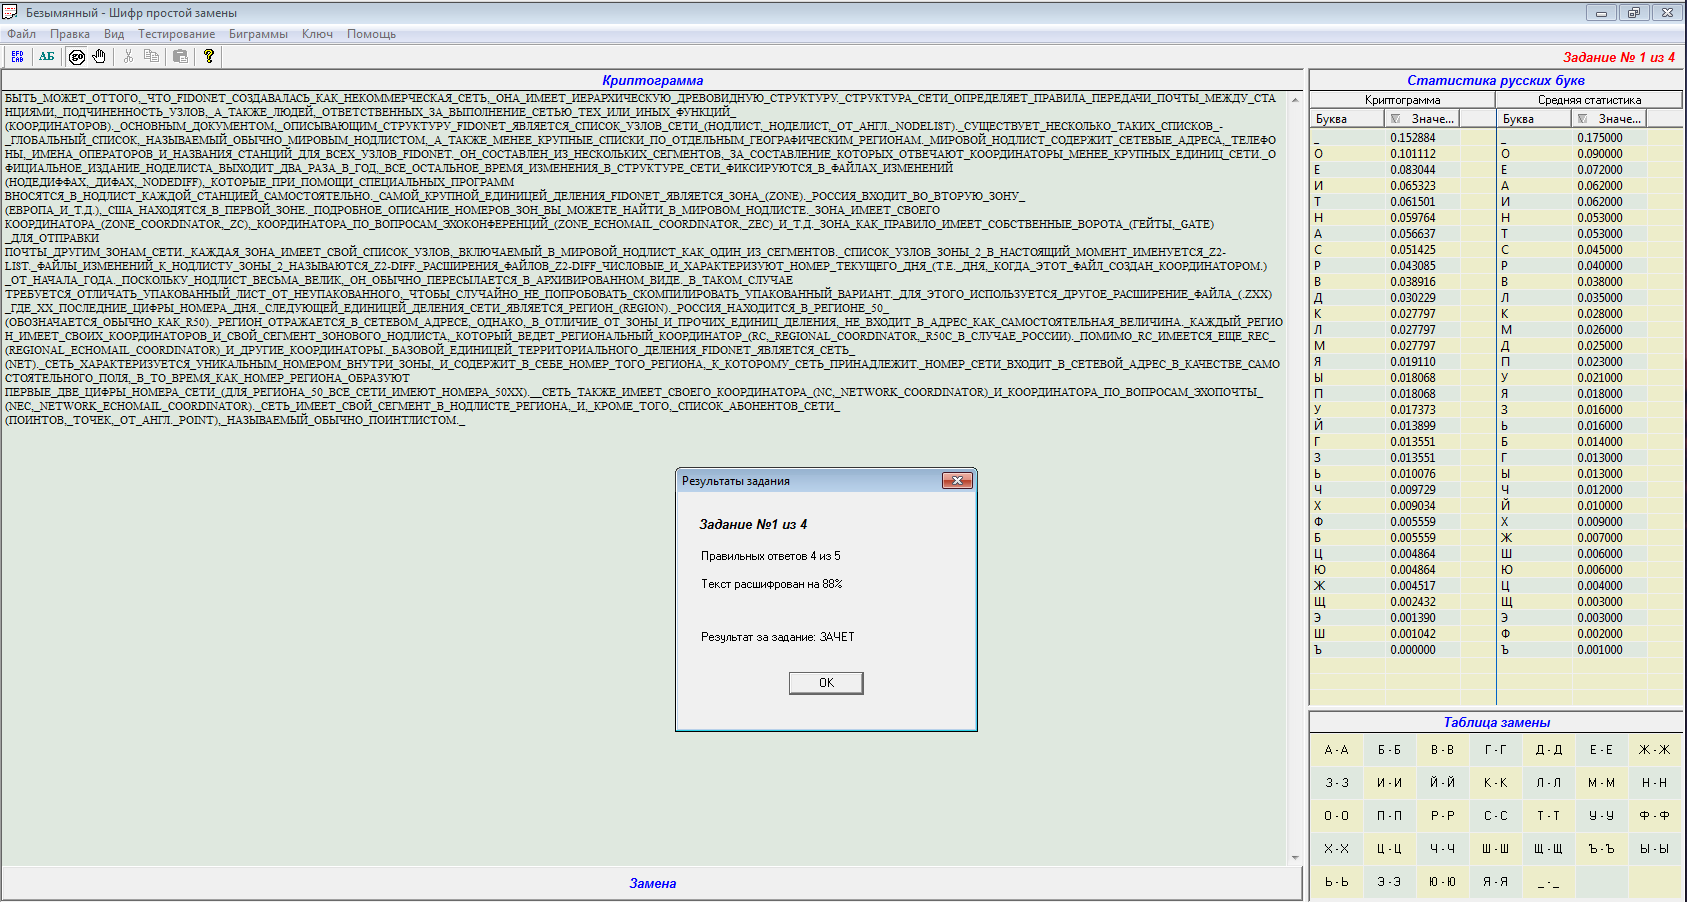
\includegraphics[scale=0.3]{pics/1_2.png}

        "Текст 1, результаты теста"
    \end{center}
    \begin{center}
        \textbf{Ключ}
    \end{center}
    \vspace{-3em}
    \begin{center}
        \begin{tabular}{|c|c|c|c|c|c|c|c|c|c|c|c|c|c|c|c|c|c|c|c|c|c|c|c|c|c|}
            \hline
            а & б & в & г & д & е & ж & з & и & й & к & л & м & н & о & п & р & с & т & у & ф & х & ц & ч & ш & щ  \\
            \hline
            э & к & р & з & с & х & м & ф & н & и & ч & г & й & в & ш & ц & р &\_ & а & д & п & л & ж & т & щ & ю   \\
            \hline
        \end{tabular}
    \end{center}
    \begin{tabular}{|c|c|c|c|c|c|c|}
        \hline
        ъ & ы & ь & э & ю & я & \_ \\
        \hline
        б & у & ъ & я & е & о & ь \\
        \hline
    \end{tabular}\\

    \newpage
    \begin{center}
        \textbf{Текст 2}
    \end{center}
    \begin{center}
        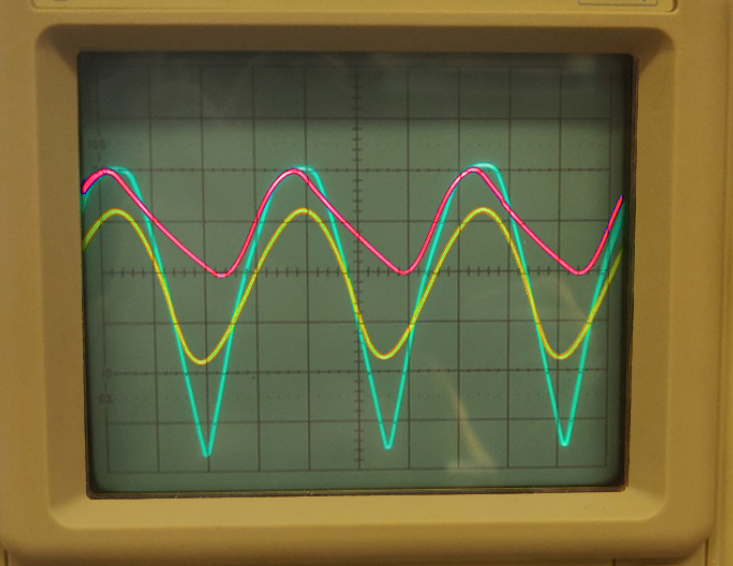
\includegraphics[scale=0.3]{pics/2.png}

        "Текст 2, зашифрованный"
    \end{center}
    \begin{center}
        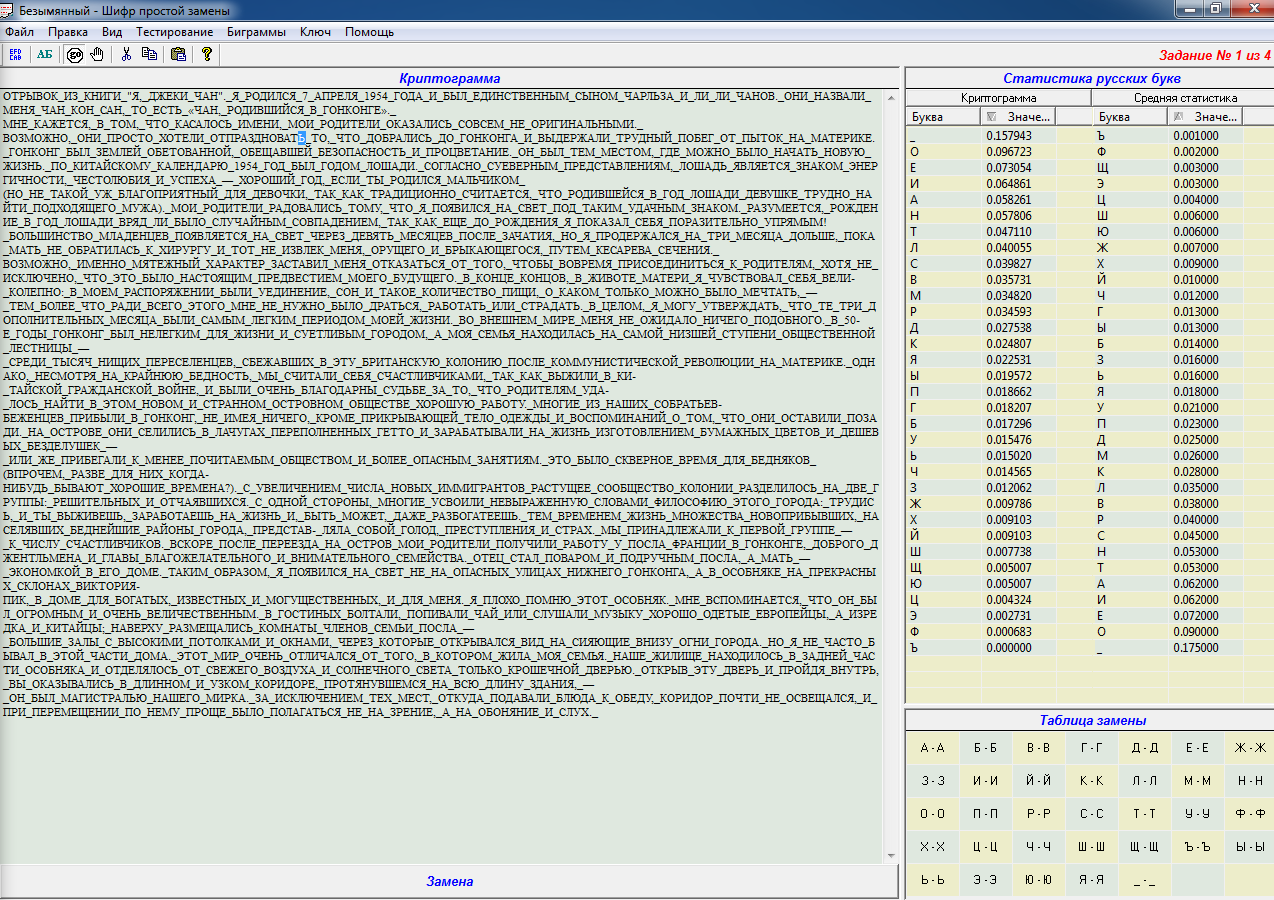
\includegraphics[scale=0.3]{pics/2_1.png}

        "Текст 2, расшифрованный"
    \end{center}
    \begin{center}
        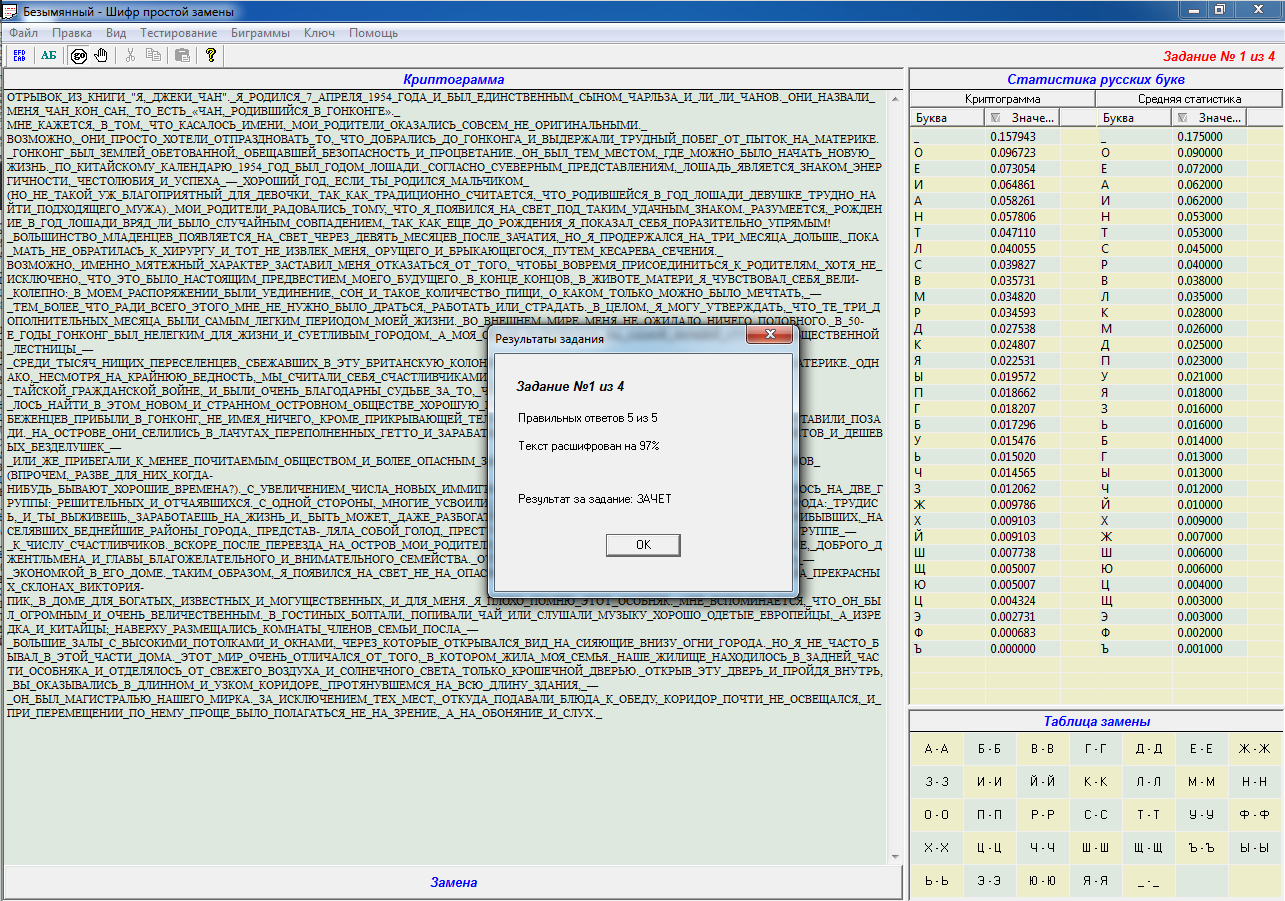
\includegraphics[scale=0.3]{pics/2_2.png}

        "Текст 2, результаты теста"
    \end{center}
    \begin{center}
        \textbf{Ключ}
    \end{center}
    \vspace{-3em}
    \begin{center}
        \begin{tabular}{|c|c|c|c|c|c|c|c|c|c|c|c|c|c|c|c|c|c|c|c|c|c|c|c|c|c|}
            \hline
            а & б & в & г & д & е & ж & з & и & й & к & л & м & н & о & п & р & с & т & у & ф & х & ц & ч & ш & щ  \\
            \hline
            ь & м & л & ж & о & п & к & с & з & в & й & ц & ы & я & д & р & а & и & щ & х & ф & б & э & ю & г & ш   \\
            \hline
        \end{tabular}
    \end{center}
    \begin{tabular}{|c|c|c|c|c|c|c|}
        \hline
        ъ & ы & ь & э & ю & я & \_ \\
        \hline
        н & ч & т & е & у & ъ & ы \\
        \hline
    \end{tabular}\\

    \newpage
    \begin{center}
        \textbf{Текст 3}
    \end{center}

    \begin{center}
        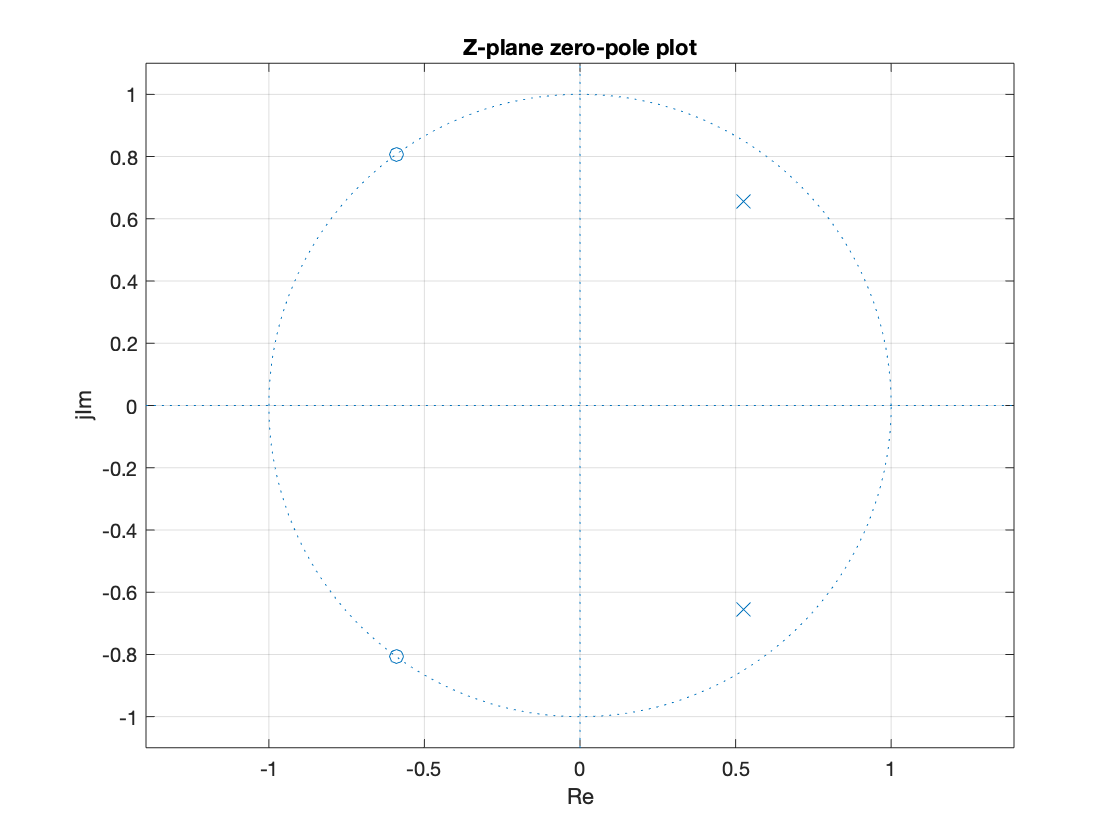
\includegraphics[scale=0.3]{pics/3.png}

        "Текст 3, зашифрованный"
    \end{center}
    \begin{center}
        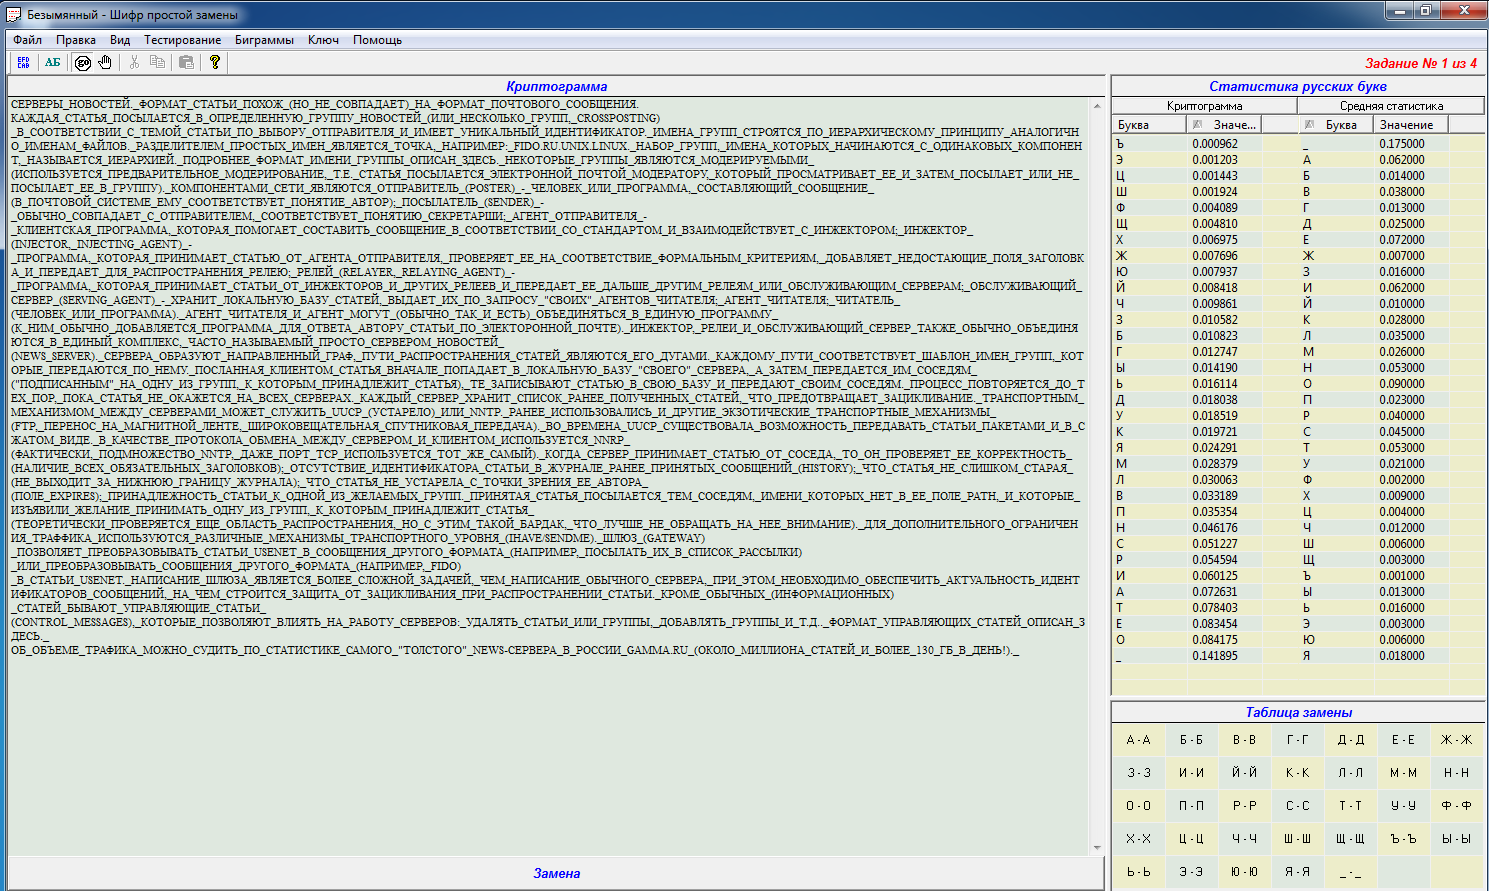
\includegraphics[scale=0.3]{pics/3_1.png}

        "Текст 3, расшифрованный"
    \end{center}
    \begin{center}
        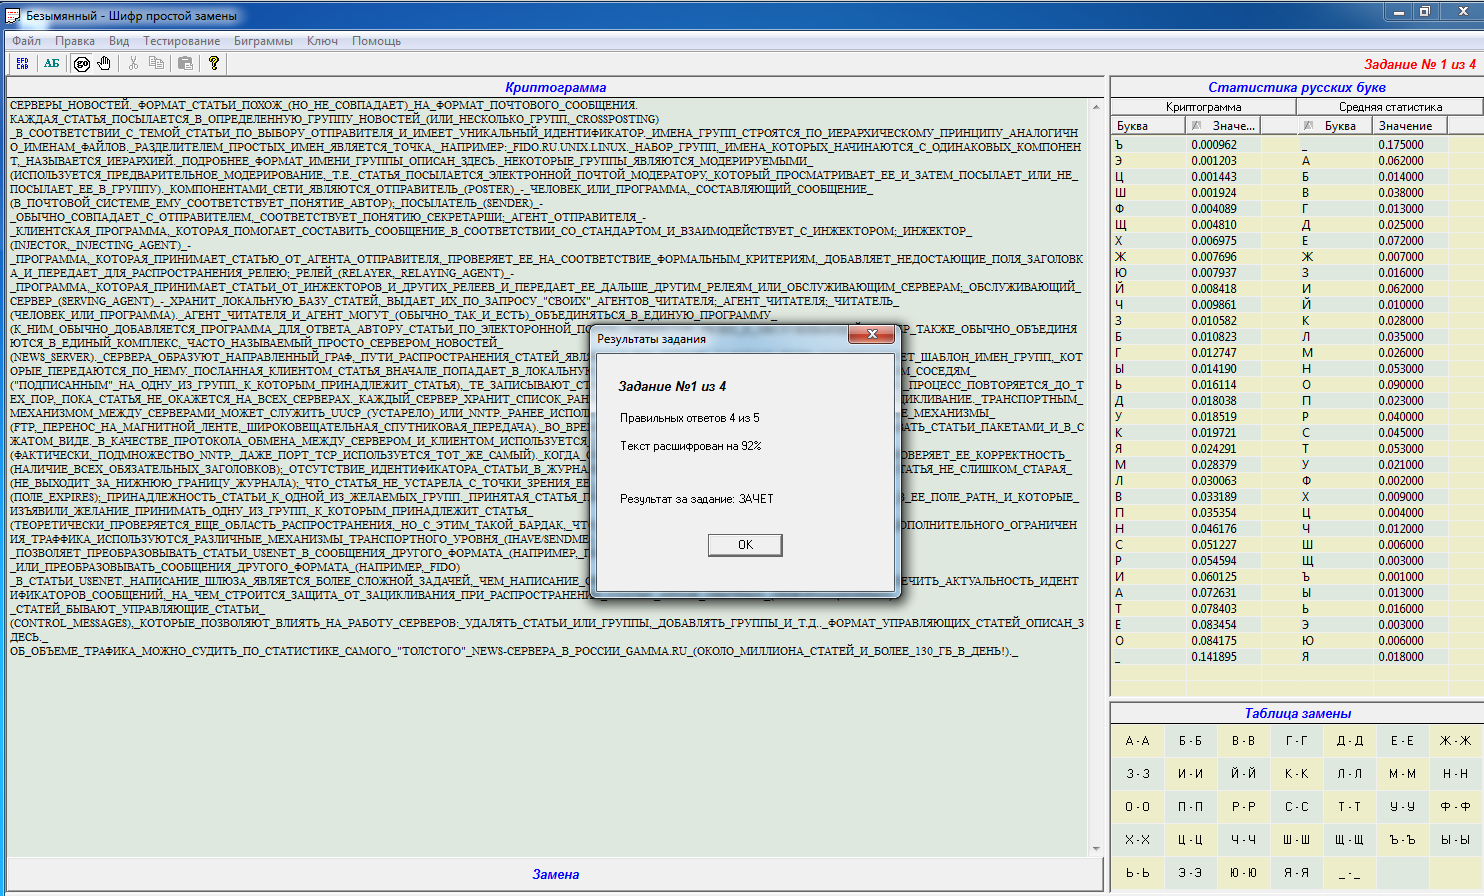
\includegraphics[scale=0.3]{pics/3_2.png}

        "Текст 3, результаты теста"
    \end{center}
    \begin{center}
        \textbf{Ключ}
    \end{center}
    \vspace{-3em}
    \begin{center}
        \begin{tabular}{|c|c|c|c|c|c|c|c|c|c|c|c|c|c|c|c|c|c|c|c|c|c|c|c|c|c|}
            \hline
            а & б & в & г & д & е & ж & з & и & й & к & л & м & н & о & п & р & с & т & у & ф & х & ц & ч & ш & щ \\
            \hline
            г & х & я & л & ф & п & з & с & в & ы & м & э & у & т & б & н & й & р & ж &\_ & и & к & е & о & ч & ц \\
            \hline
        \end{tabular}
    \end{center}
    \begin{tabular}{|c|c|c|c|c|c|c|}
        \hline
        ъ & ы & ь & э & ю & я & \_ \\
        \hline
        щ & ш & д & ю & ь & а & ъ \\
        \hline
    \end{tabular}\\



    \textbf{Выводы}
    \begin{enumerate}
        \item Шифр замены на первый взгляд кажется невозможным для расшифровки.
        Однако, благодаря тому, что мы знаем среднюю статистику букв русского алфавита,
        данный шифр можно достаточно просто расшифровать. Расшифровка происходит путем,
        сопоставления средней статистики букв в алфавите и в криптограмме, и последующей
        заменой.
        \item Для увеличения стойкости нужно вместо шифра простой замены применить шифр
        колонной замены.

    \end{enumerate}
\end{document}